\documentclass[a4paper, 12pt]{article}

\usepackage[T2A]{fontenc}
\usepackage[utf8]{inputenc}
\usepackage[english,russian]{babel}
\usepackage[left=15mm, top=20mm, right=15mm, bottom=20mm, nohead, nofoot]{geometry}

\usepackage{hyperref}
\usepackage{graphicx}
\usepackage{wrapfig}
\usepackage{afterpage}
\usepackage{amsmath, amsfonts, amssymb, amsthm, mathtools}
\author{Хомутов Андрей, группа Б06-903}
\title{ВПВ по курсу "Электричество и магнетизм" \\ Конденсатор на высоких частотах}
\date{22 декабря 2020 г.}
%%%%%%%%%%%%%%%%%%%%%%%%%%%%%%%%%%%%%%%%%%%%%%%%%%%%%%%%%%%%%%%%%%%%%%%%%
\usepackage{graphicx, wrapfig, subcaption, setspace, booktabs}
\usepackage[protrusion=true, expansion=true]{microtype}
\usepackage[english]{babel}
\usepackage{sectsty}
\usepackage{url, lipsum}
\newcommand{\HRule}[1]{\rule{\linewidth}{#1}}
\onehalfspacing
\setcounter{tocdepth}{5}
\setcounter{secnumdepth}{5}
%%%%%%%%%%%%%%%%%%%%%%%%%%%%%%%%%%%%%%%%%%%%%%%%%%%%%%%%%%%%%%%%%%%%%%%%%


\begin{document}

\title{ \normalsize \textsc{Лабораторная работа по общей физике}
		\\ [4.0cm]
		\HRule{0.5pt} \\ [0.3cm]
		\LARGE \textbf{{Тепловое излучение}}
		\HRule{0.5pt} \\ [0.1cm]
		\normalsize  \vspace*{18\baselineskip}}

\date{}

\author{Рыбкина Елизавета, Б06-903 \\
Хомутов Андрей, Б06-903 \\
ФБМФ, 2021\\ }

\maketitle
\thispagestyle{empty}
\newpage
%%%%%%%%%%%%%%%%%%%%%%%%%%%%%%%%%%%%%%%%%%%%%%%%%%%%%%%%%%%%%%%%%%%%%%%%%
\section*{Цель работы}
\begin{enumerate}
    \item При помощи модели абсолютно чёрного тела проведение измерения температуры оптическим пирометром с исчезающей нитью и термопарой
    \item Исследование излучение накалённых тел с различной испускательной способностью
    \item Определение постоянных Планка и Стефана-Больцмана
\end{enumerate}

\section*{В работе используются:}
\begin{itemize}
    \item оптический пирометр
    \item модель абсолютно чёрного тела
    \item образцы колец
    \item вольфрамовая лампа
    \item неоновая лампа
    \item блок питания
    \item цифровые вольтметры
\end{itemize}

\section{Теоретические часть}
Для измерения температуры разогретых тел, удалённых от наблюдателя, применяют методы оптической пирометрии, основанные на использовании зависимости испускательной способности исследуемого тела от температуры. Различают три температуры, функционально связанные с истинной термодинамической температурой и излучательной способностью тела: радиационную $T_{rad}$, цветовую $T_{col}$ и яркостную $T_b_r$. \par
В работе измеряется яркостная температура. \textbf{Яркостная температура} - это температура абсолютно чёрного тела, при которой его спектральная испускательная способность равна спектральной испускательной способности исследуемого тела при той же длине волны.
 Измерение яркостной температуры раскалённого тела производится при помощи оптического пирометра с исчезающей нитью, основанного на визуальном сравнении яркости раскалённой нити с яркостью изображения исследуемого тела. \par
Яркостная температура тела всегда ниже его термодинамической температуры. Это связано с тем, что любое нечёрное тело излучает меньше, чем АЧТ при той же температуре. Зависимость между яркостной и термодинамической температурами вольфрама приведена на рис. 1

\begin{figure}[h]
    \centering
    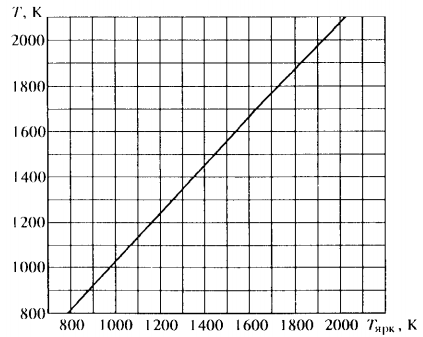
\includegraphics[width=10cm]{fig2.PNG}
    \caption{График зависимости $T = f(T_b_r)$ для вольфрама}
    \label{fig:vac}
\end{figure}

По результатам измерений мощности излучения вольфрамовой нити можно судить о справедливости закона Стефана-Больцмана. Если бы нить излучала как АЧТ, то баланс потребляемой и излучаемой энергии определялся бы соотношением 
\begin{equation}
    W = \sigma S (T^4 - T_0^4),
\end{equation}
где $W$ - потребляемая нитью электрическая мощность, $S$ - площадь излучающей поверхности нити, $T$ - температура нити, $T_0$ - температура окружающей среды. Однако вольфрамовая нить излучает как серое тел, и излучение её ослаблено по сравнению с АЧТ в $\varepsilon_T$ раз для любой волны при данной температуре тела Т. Тогда предположив, что нить излучает как серое тело и с учётом того, что $T_0 \ll T$, выражение (1) можно переписать в виде
\begin{equation}
    W = \varepsilon_T S \sigma T^4
\end{equation}
В справедливости закона Стефана-Больцмана можно убедиться, построив график зависимости $W(T)$ в логарифмическом масштабе и по углу наклона определить показатель степени $n$ исследуемой температурной зависимости. В пределах погрешности показатель степени должен быть близок к четырём. \par
Также из формулы (2) можно определить постоянную Стефана-Больцмана.

\newpage

\section{Экспериментальная установка}

\begin{figure}[h]
    \centering
    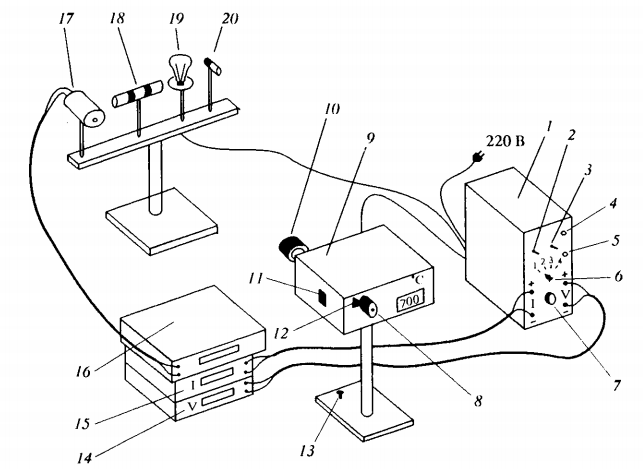
\includegraphics[width=11cm]{fig1.PNG}
    \caption{Схема экспериментальной установки: 1 - блок питания; 2 - тумблер включения питания образцов; 3 - тумблер нагрева нити пирометра; 4 - кнопка "Нагрев нити"; 5 - кнопка "охлаждение нити"; 6 - тумблер переключения образцов; 7 - регулятор мощности нагрева образцов; 8 - окуляр пирометра; 9 - корпус пирометра; 10 - объектив пирометра; 11 - переключение диапазонов; 12 - ручка смещения красного светофильтра; 13 - регулировочный винт; 14 - вольтметр (напряжение на лампе накаливания); 15 - амперметр (ток через образцы); 16 - вольтметр в цепи термопары; 17 - модель АЧТ; 18 трубка с кольцами из материалов с различной излучательной способностью; 19 - лампа накаливания; 20 - неоновая лампочка}
    \label{fig:vac}
\end{figure}

Исследуемые в работе образцы:
\begin{itemize}
    \item \textbf{модель абсолютно чёрного тела} - керамическая трубка, закрытая с одного конца и окружённая для теплоизоляции внешним кожухом. Температура в трубке измеряется с помощью термопары хромель-алюмель
    \item \textbf{керамическая трубка с набором колец из различных материалов}, нагреваемая изнутри нихромовой спиралью. Материалы колец имеют различную излучательную способность
    \item \textbf{вольфрамовая нить электрической лампочки}
\end{itemize}

\newpage

\section{Практическая часть}
\subsection{Изучение работы оптического пирометра}

С помощью пирометра измеряется температура модели АЧТ и проводится сравнение её значения  со значением температуры, измеренной при помощи термопарного термометра
\begin{enumerate}
    \item Настроим пирометр, прогреем его нить. Прогреем модель АЧТ.
    \item Введём красный светофильтр пирометра. Изменяя ток через нить пирометра, добьёмся исчезновения нити на фоне изображения раскалённой поверхности дна АЧТ. Проверим корректность измерений: температура на пирометре не должна сильно отличаться от температуры АЧТ, измеренной термопарой. 
    \item 


Видим, что разница в показаниях приборов не превышает 10\%
\end{enumerate}

\subsection{Измерение яркостной температуры тел}
Хотим проверить, что разные тела, накалённые до одинаковой термодинамической температуры, имеют различную яркостную температуру
\begin{enumerate}
    \item Прогреем керамическую трубку с образцами до красного каления.
    \item Измерим яркостную температуру колец
    \item Температура левого кольца $798 \pm 2 \text{ }^\circ C$, правого - $774 \pm 4 \text{ }^\circ C$
Несовпадение яркостной температуры у различных тел, имеющих одинаковую термодинамическую температуру, объясняется связью этих величин через спектральный коэффициент поглощения, разнящийся от тела к телу.
\end{enumerate}

\subsection{Проверка закона Стефана-Больцмана}
\begin{enumerate}
    \item Постепенно увеличивая накал нити лампы, начиная со слабого тёмно-красного накала до 1900$^{\circ}$C, будем измерять пирометром яркостную температуру нити, а также значение силы тока и напряжения на ней. Результаты измерений занесём в таблицу 1. Определим также по значениям яркостной температуры нити её термодинамическую температуру, используя рис. 1.

\item Представим зависимость $W=f(T)$ в логарифмическом масштабе как $\ln(W) = \ln(\varepsilon_T \sigma S) + n \ln(T)$ По углу наклона графика можно определить показатель степени температуры в законе Стефана-Больцмана. В итоге $n = 3,91 \pm 0,18$, что согласуется с теоретической зависимостью.

\begin{figure}[h]
    \centering
    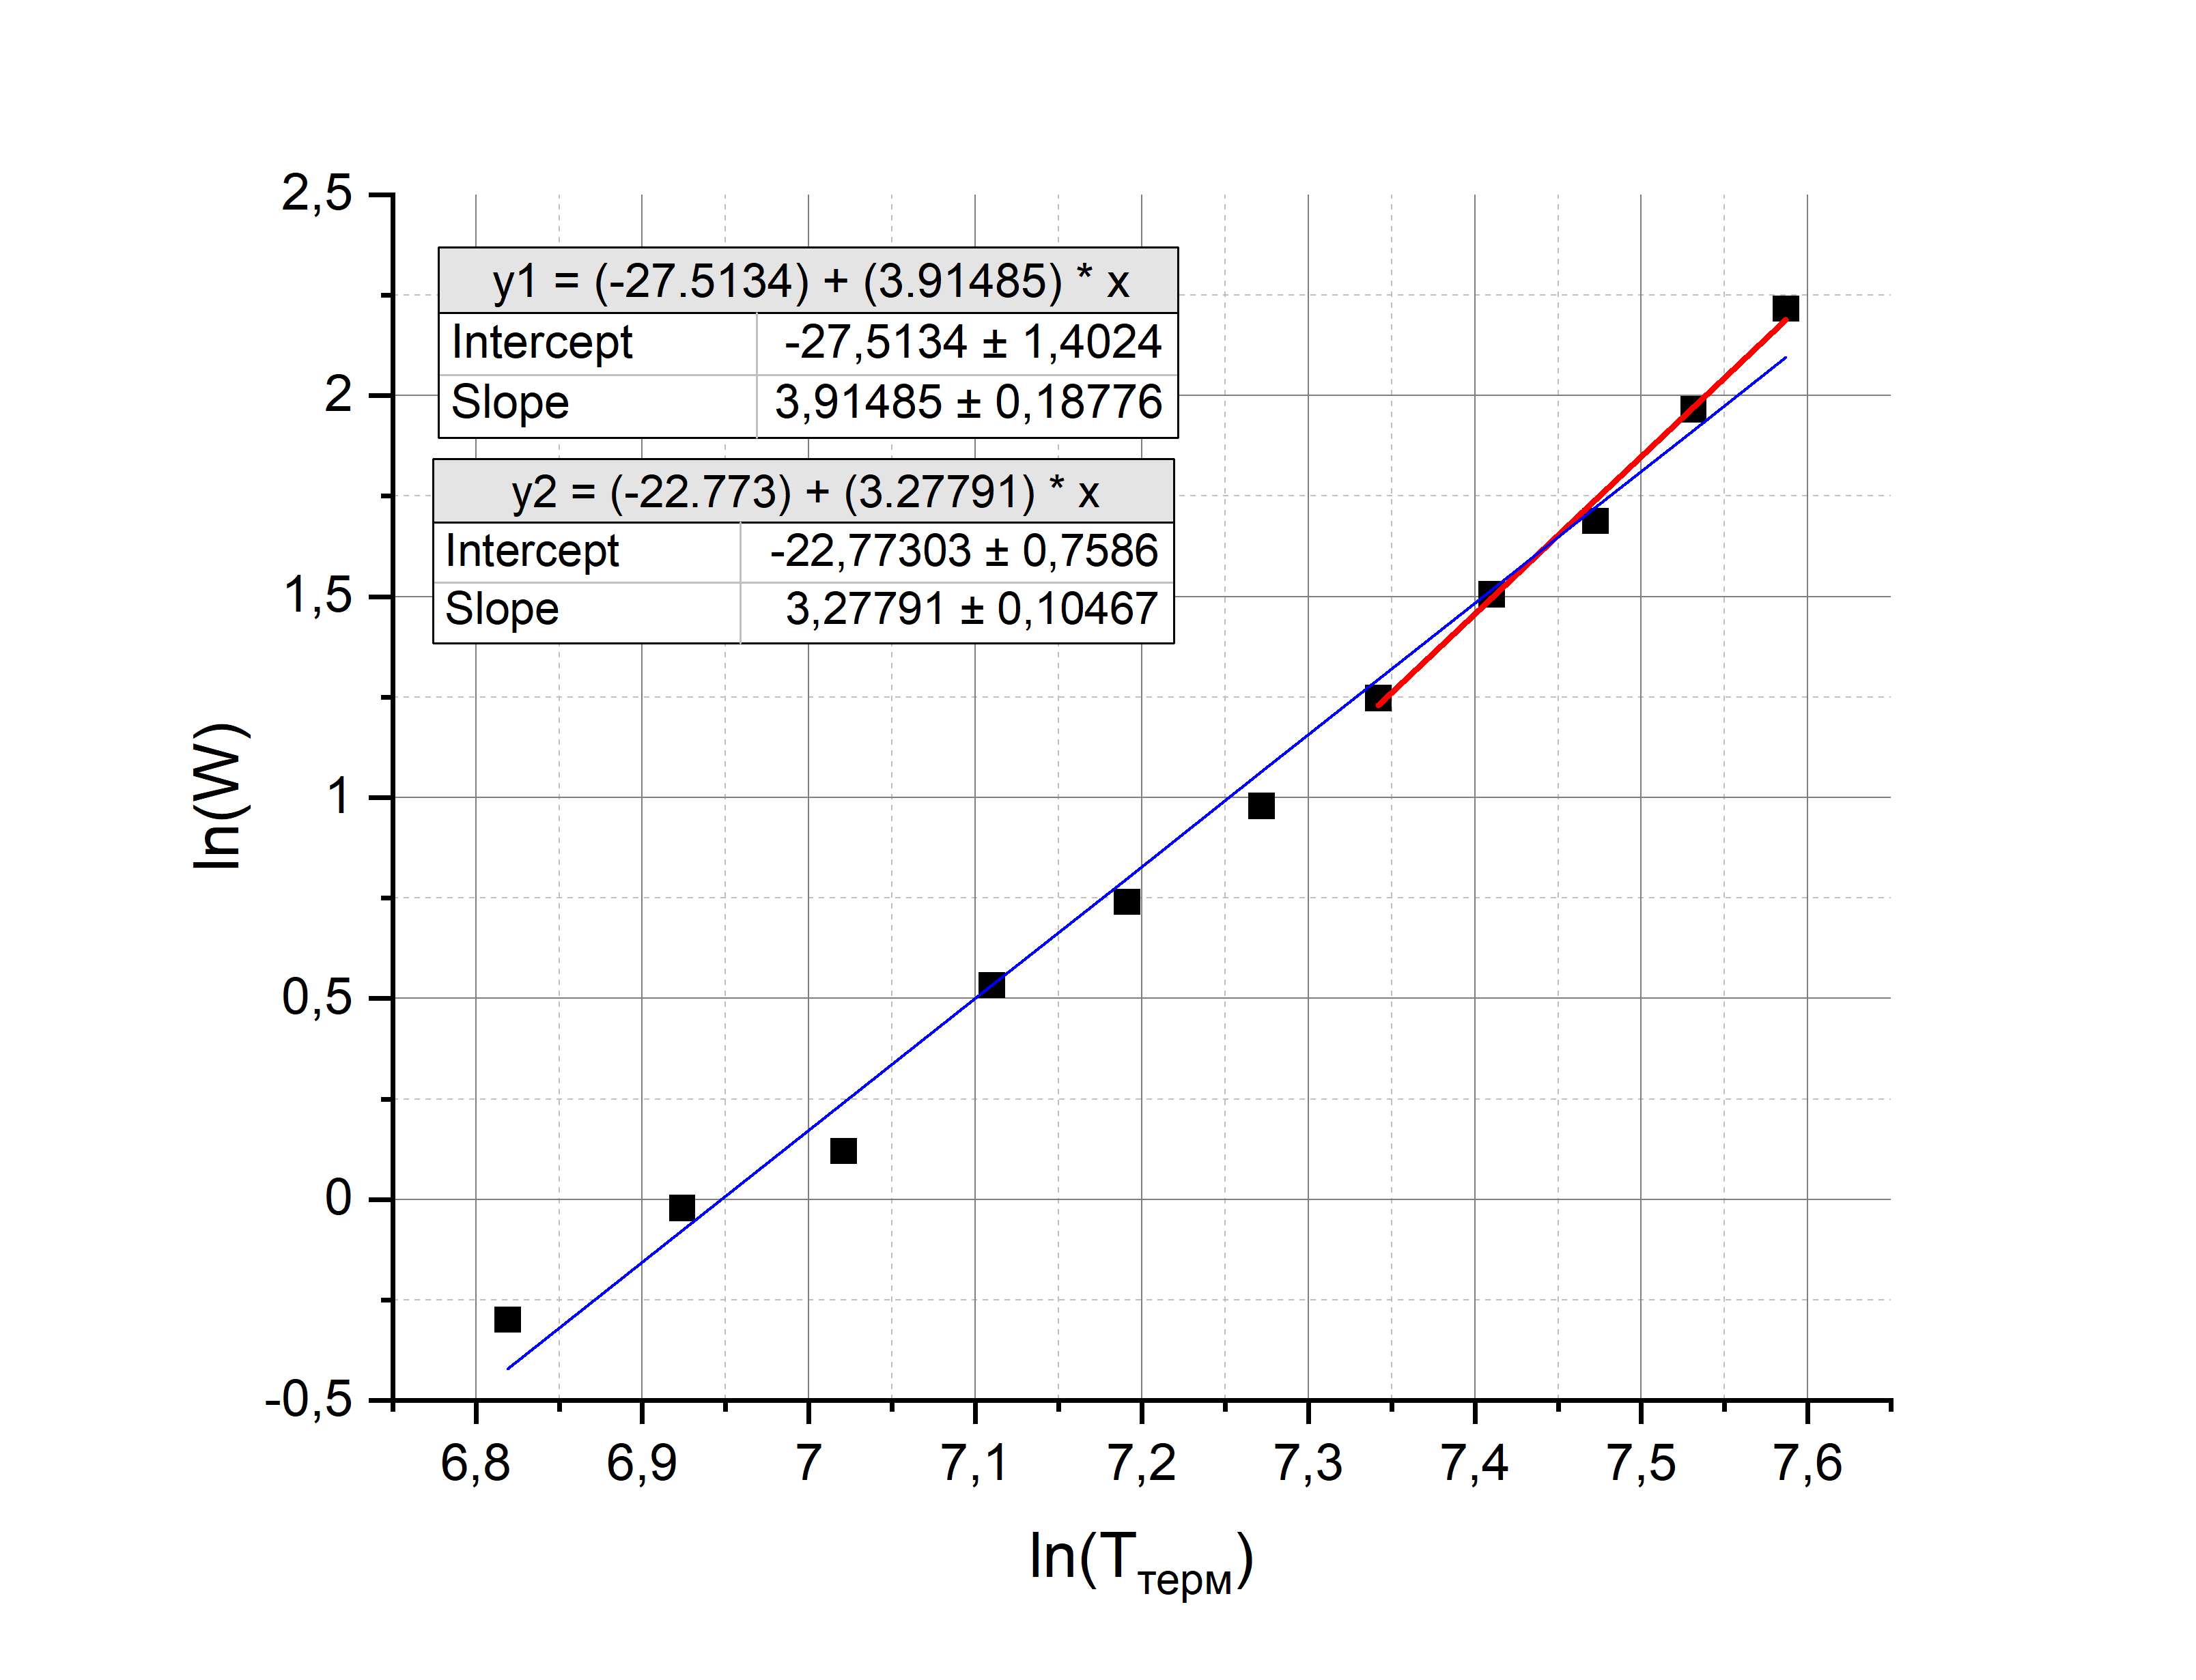
\includegraphics[width=\textwidth]{W_T.png}
    \caption{Зависимость мощности лампы от её термодинамической температуры, логарифмический масштаб}
    \label{fig:vac}
\end{figure}

\begin{table}[h]
    \centering
    \begin{center}
    \caption{Зависимость мощности, выделяемой на лампе, от температуры нити накала}
    \end{center}
    \vspace{0.1cm}
    \label{tab:my_label}
\begin{tabular}{|c|c|c|c|c|}
\hline
T(ярк), С & Т(терм), С & I, A  & V, В  & N, Вт \\ \hline
908       & 915        & 0,495 & 1,499 & 0,74  \\ \hline
1003      & 1016       & 0,535 & 1,83  & 0,98  \\ \hline
1100      & 1120       & 0,557 & 2,026 & 1,13  \\ \hline
1198      & 1224       & 0,63  & 2,705 & 1,70  \\ \hline
1295      & 1327       & 0,672 & 3,12  & 2,10  \\ \hline
1400      & 1439       & 0,725 & 3,672 & 2,66  \\ \hline
1498      & 1544       & 0,791 & 4,401 & 3,48  \\ \hline
1600      & 1652       & 0,863 & 5,224 & 4,51  \\ \hline
1700      & 1759       & 0,917 & 5,901 & 5,41  \\ \hline
1800      & 1866       & 1,008 & 7,085 & 7,14  \\ \hline
1900      & 1972       & 1,105 & 8,304 & 9,18  \\ \hline
\end{tabular}
\end{table}   

\item Определим постоянную Стефана-Больцмана, используя значение термодинамической температуры 1870$^{\circ}$C и соответствующую мощность ($\varepsilon_T(1900) \approx 0.236$, $S = 0.36$ см$^2$):
\begin{center}
    $\sigma = \frac{W}{\varepsilon_T S T^4} = 8.3 \cdot 10^{-12}$ Вт/(см$^2 \cdot$ K$^4$)
\end{center}
Еще  можно попробовать определить постоянную Стефана-Больцмана, используя построенный график:
\begin{center}
    $\ln(\varepsilon_t \sigma S) = -27.5134$ \\
    \\
    $\sigma = \frac{e^{-27.5134}}{\varepsilon_T S} = 1.3 \cdot 10^{-12}$ Вт/(см$^2 \cdot$ K$^4$)
\end{center}

Видно что оба метода дают ошибку меньше чеи на порядок, однако первый способ позволил получить практически справочное значение
\begin{center}
    $\sigma_0= 5.67\cdot 10^{-12}$ Вт/(см$^2 \cdot$ K$^4$)
\end{center}

\item Оценим значение постоянной Планка:
\begin{center}
    $h = \sqrt[3]{\frac{2 \pi^5 k_B^4}{15 c^2 \sigma}} \approx 8.5 \dot 10^{-34}$ Дж$\cdot$с
\end{center}

\end{enumerate}

\subsection{Измерение яркостной температуры неоновой лампочки}
Термодинамическая температура неоновой лампочки примерно равна комнатной, и не соответствует её яркостной температуре ($\approx$ 846$^{\circ}$C). На самом деле механиз излучения неоновой лампы носит принципиально иной характер в сравнении с моделью АЧТ и является следствием электронных переходов между энергетическими уровнями.

\section{Вывод}
В работе были изучены тепловые излучения АЧТ и серых тел (колец) с помощью оптического пирометра, доказана корректность его показаний для определения яркостной температуры.

Можно было убедится что для тел с одинаковой термодинамической температурой, температура яркостная может различаться, что объясняется различными коэффициентами поглощения веществ.

Была проверена справедливость закона Стефана-Больцмана, с большой точностью были проверены показатель температуры в законе, постоянная Стефана-Больцмана и постоянная Планка.

Также мы убедились что для неоновой лампы имеющей комнатную термодинамическую температуру, яркостная составила около 900 градусов. Такое большое различие объясняется узким спектром испускания неона.
\end{document}



%%%%%%%%%%%%%%%%%%%%%%%%%%%%%%%%%%%%%%%%%%%%%%%%%%%%%%%%%%%%%%%%%%%%%%%%%
 \section{Выводы}
\begin{enumerate}
    \item 
    \item 

\end{enumerate}

\end{document}

\begin{table}[h!]
\begin{center}
\caption{...}
\begin{tabular}{|c|c|c|c|c|}

\end{tabular}
\end{center}
\end{table}


\begin{figure}[h!]
    \begin{center}
    \includegraphics[width=0.8\textwidth]{xxx.png}
    \end{center}
    \caption{...}
\end{figure}

\begin{figure}[h!] %% ШАБЛОН ДЛЯ ДВУХ КАРТИНОК
\begin{center}
\begin{minipage}[h]{0.40\linewidth}
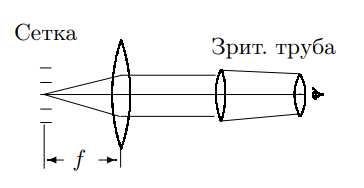
\includegraphics[width=1\linewidth]{plus_lens.PNG}
\caption{...} %% подпись к рисунку
\label{ris:experimoriginal} %% метка рисунка для ссылки на него
\end{minipage}
\hfill 
\begin{minipage}[h]{0.40\linewidth}
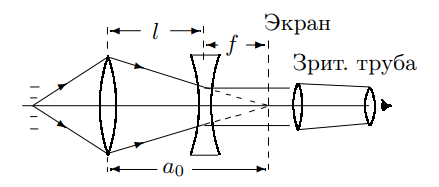
\includegraphics[width=1\linewidth]{minus_lens.PNG}
\caption{..}
\label{ris:experimcoded}
\end{minipage}
\end{center}
\end{figure}

\subsection{...}
\subsubsection{...}



\subsubsection{...}